\chapter{HASIL DAN PEMBAHASAN}
	\section{Hasil Implementasi}
		\subsection{Implementasi Infrastruktur Blockchain}
		Infrastruktur blockchain terdiri atas empat node \textit{Hyperledger Besu} yang saling terhubung dalam satu jaringan privat. Tiga node sebagai validator dan satu node RPC. KOnfigurasi tersebut memungkinkan transaksi berjalan secara terdistribusi, sehingga sesuai dengan kebutuhan sistem verifikasi dokumen akademik yang dikembangkan.

		\begin{figure}[h!]
			\centering
			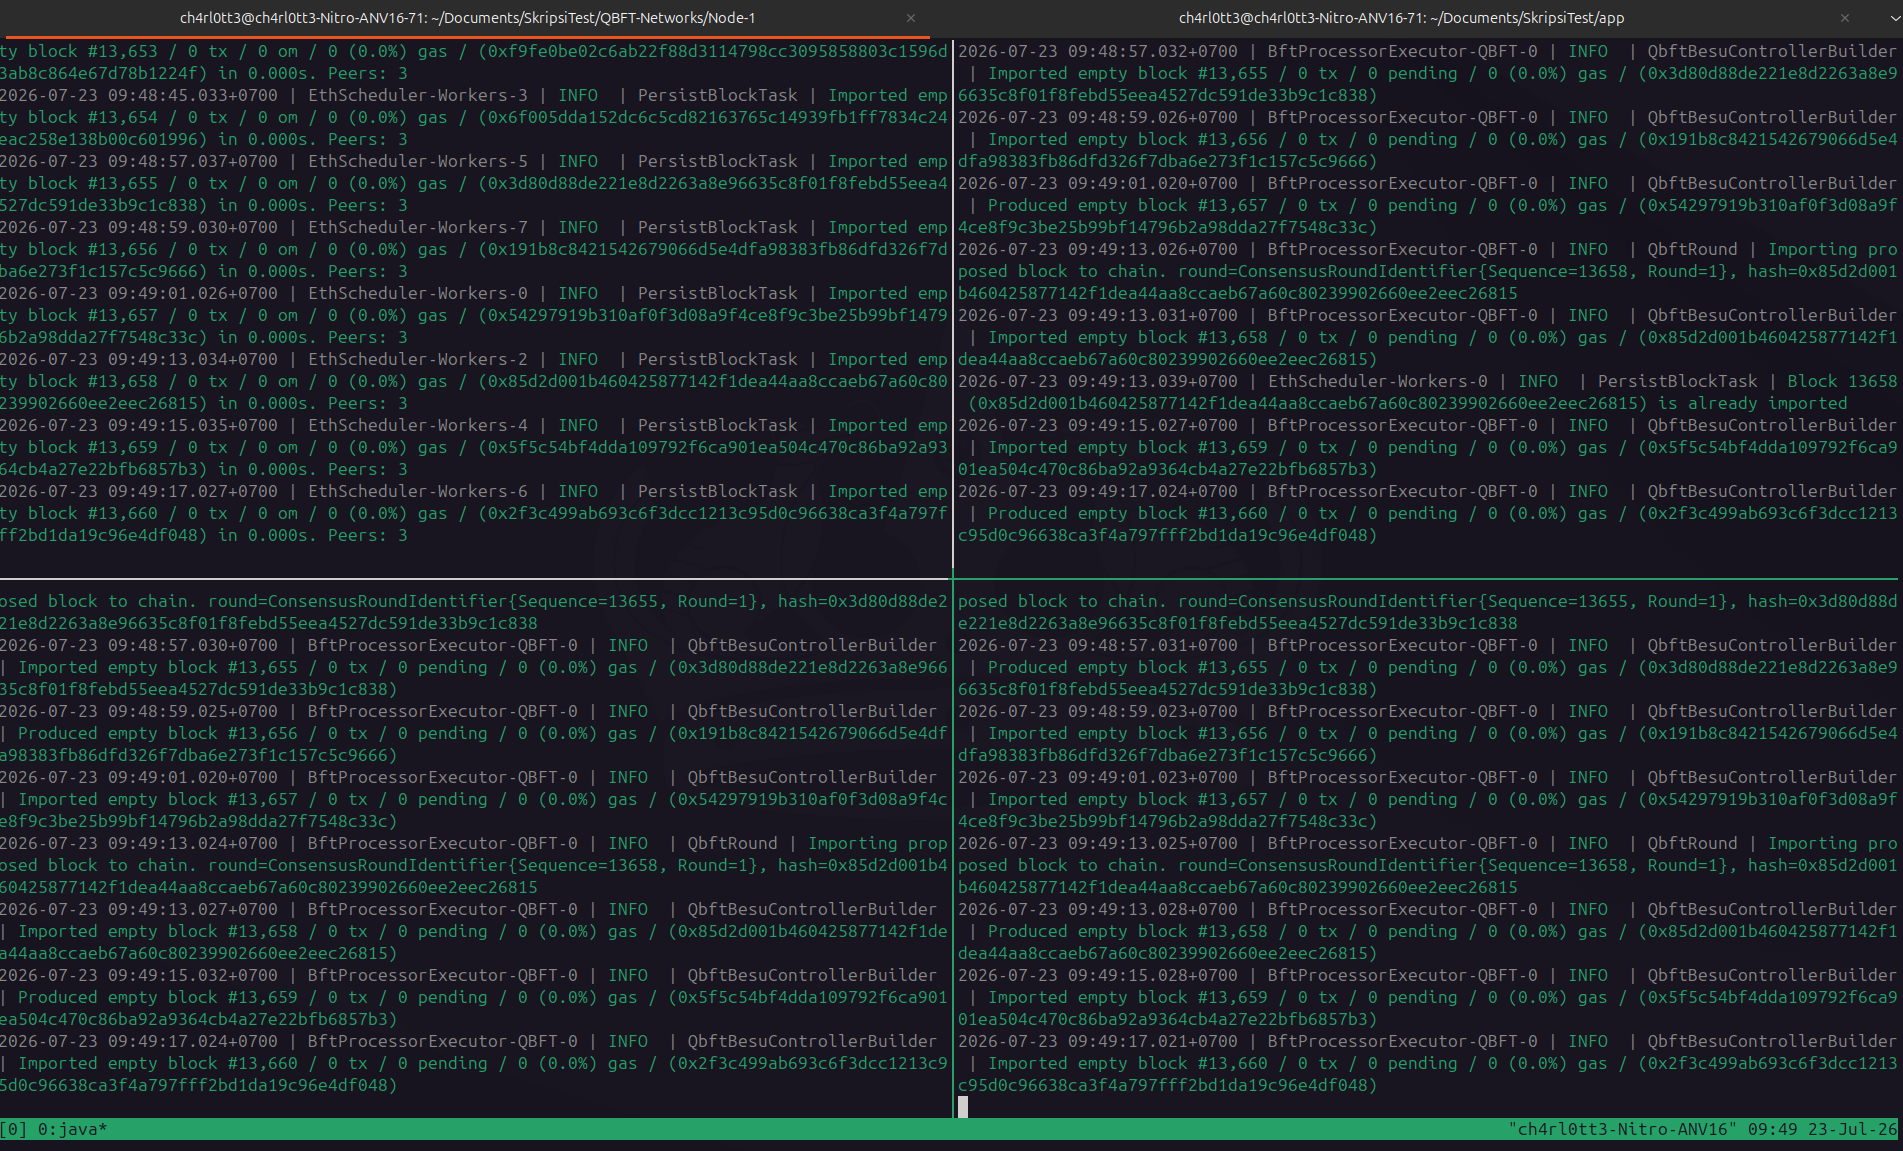
\includegraphics[width=1\textwidth]{assets/blockchain-deployed.png}
			\caption{Hyperledger  Besu Berhasil di Deploy}
			\label{fig:blockchain-deployed}
		\end{figure}

		Berdasarkan gambar \ref{fig:blockchain-deployed}, seluruh node Hyperledger  Besu dijalankan dengan status \textit{running}. Tiga node berfungsi sebagai validator yang bertugas melakukan proses konsensu QBFT, sedangkan satu node berfungsi sebagai RPC Endpoint, keberhasilan seluruh node untuk berjalan secara bersamaan menunjukan bahwa infrastuktur blockchain telah berhasil dikonfigurasi dan siap digunakan untuk penyimpanan.

		\begin{figure}[h!]
			\centering
			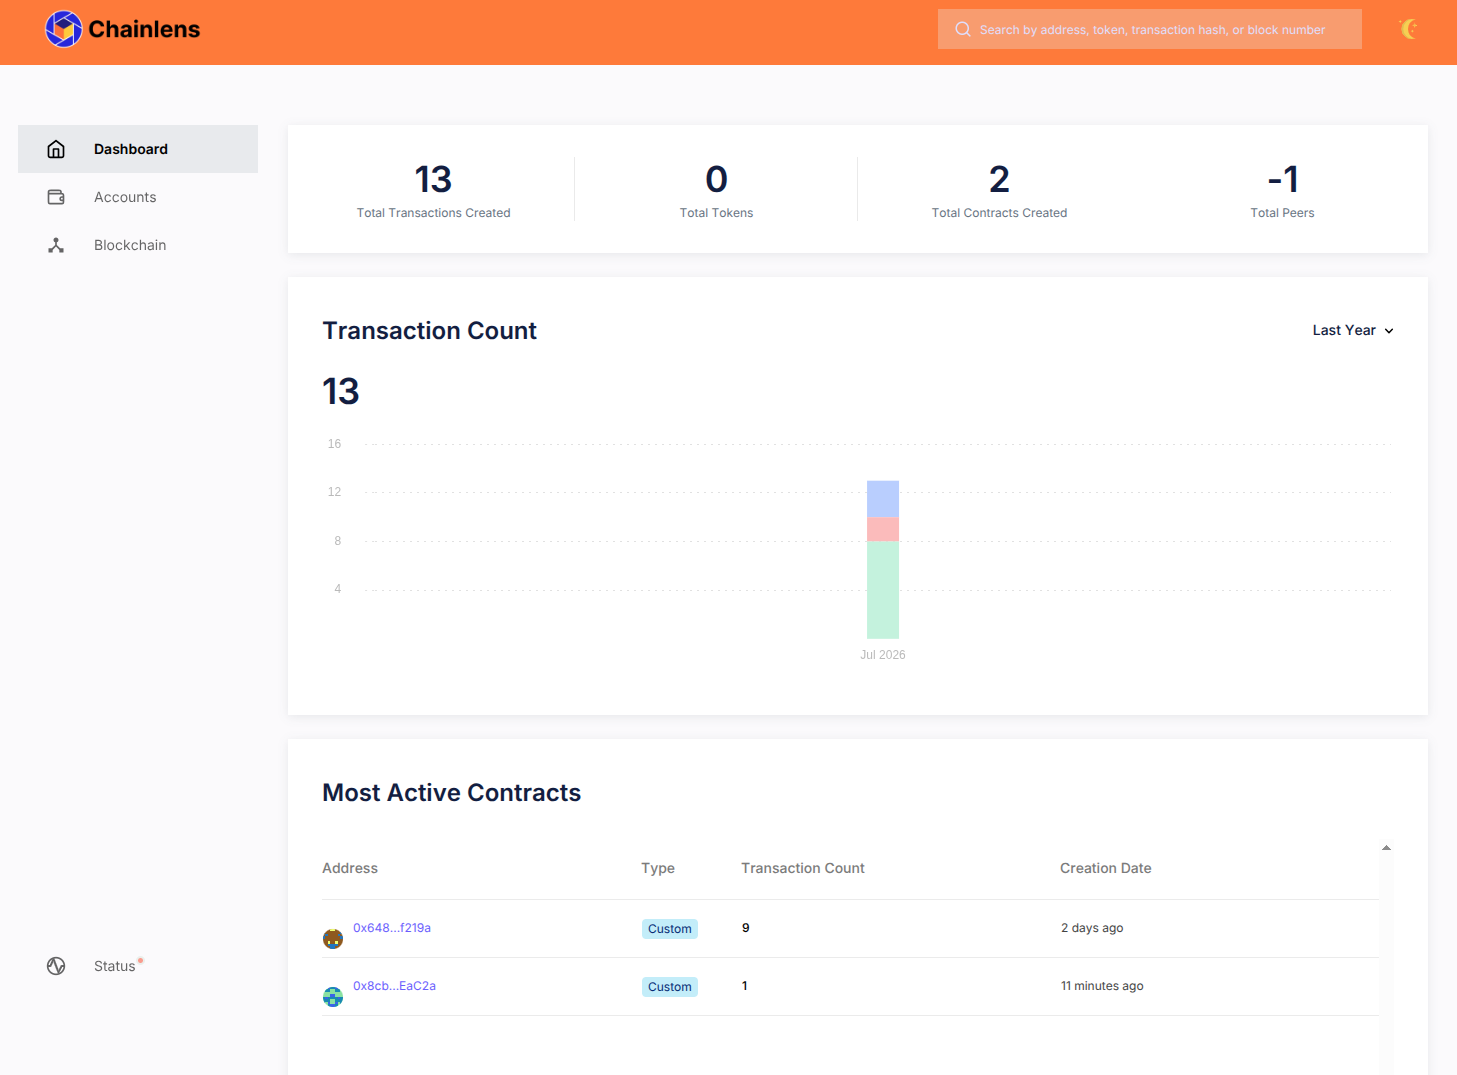
\includegraphics[width=1\textwidth]{assets/blockscout-dashboard.png}
			\caption{Halaman Utama Blockscout}
			\label{fig:blockscout-dashboard}
		\end{figure}

		Gambar \ref{fig:blockscout-dashboard} yang berhasil terhubung dengan jaringan Hyperledger Besu. Dashboard tersebut menampilkan informasi mengenai blok terbaru, jumlah transaksi, jumlah validator, serta data transaksi jaringan secara \textit{real-time}. Keberhasilan tersebut menandakan bahwasannya jaringan blockchain berjalan dan dapat diakses oleh aplikasi pendukung untuk melakukan pemantauan terhadap transaksi di jaringan.

		\subsection{Implementasi Smart Contract}
		\begin{figure}[H]
			\centering
			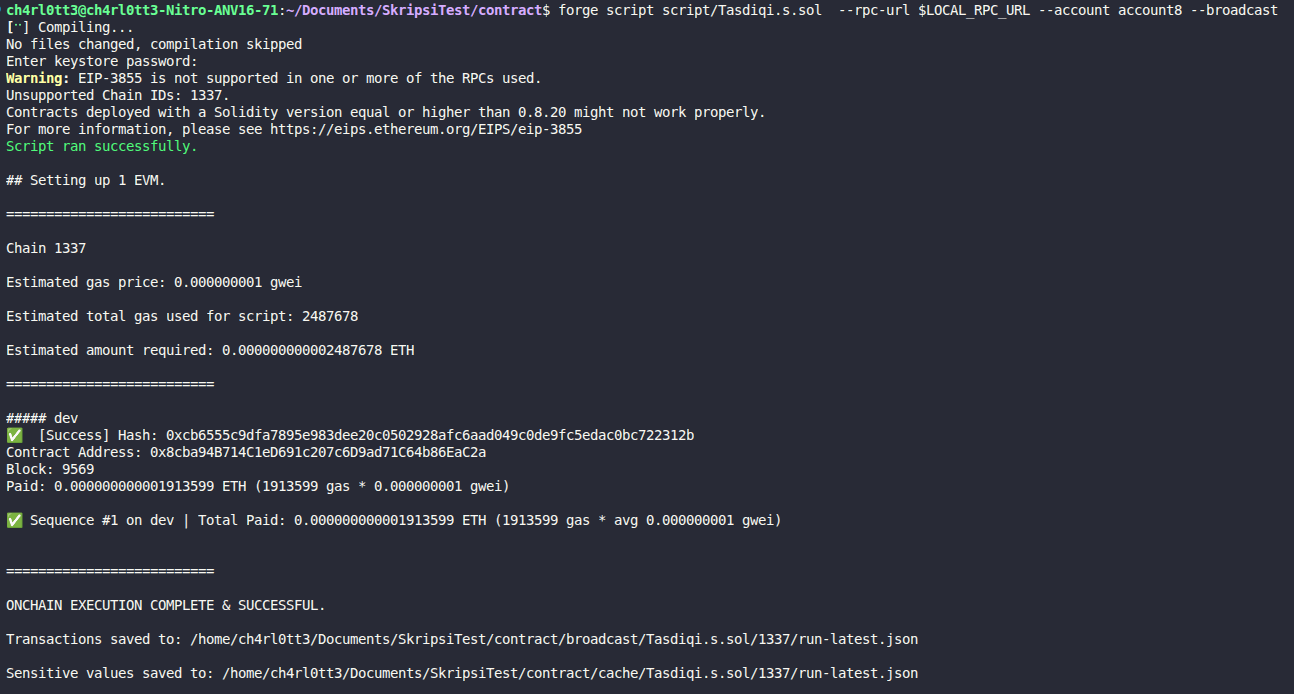
\includegraphics[width=1\textwidth]{assets/contract.png}
			\caption{smart contract berhasil dideploy}
			\label{fig:contract}
		\end{figure}

		Berdasarkan hasil pengujian pada gambar \ref{fig:contract}, proses kompilasi dan deployment smart contract ke dalam jaringan blockchain dengan \textit{Chain ID 1337} menggunakan pustaka  Foundry telah berhasil dilakukan dengan aman. Indikasi keberhasilan ini ditunjukan oleh status konfirmasi \textit{On-chain Execution Complete \& Successful}, dimana  smart contract tersebut sukses dideploy secara permanen pada alamat \textit{0x8cba94B714C1eD691c207c6d9ad71C64b86EAc2a} pada blok \textit{9569} dengan total konsumsi biaya komputasi sebesar \textit{1.913.599 gas}. Keberhasilan tahap deployment ini membuktikan bahwa infrastruktur node privat Hyperledger Besu beserta smart contract telah siap sepenuhnya untuk dihubungkan dengan lapisan API Middleware.
		
		\subsection{Implementasi Protokol EIP-712}

		\begin{figure}[H]
			\centering
			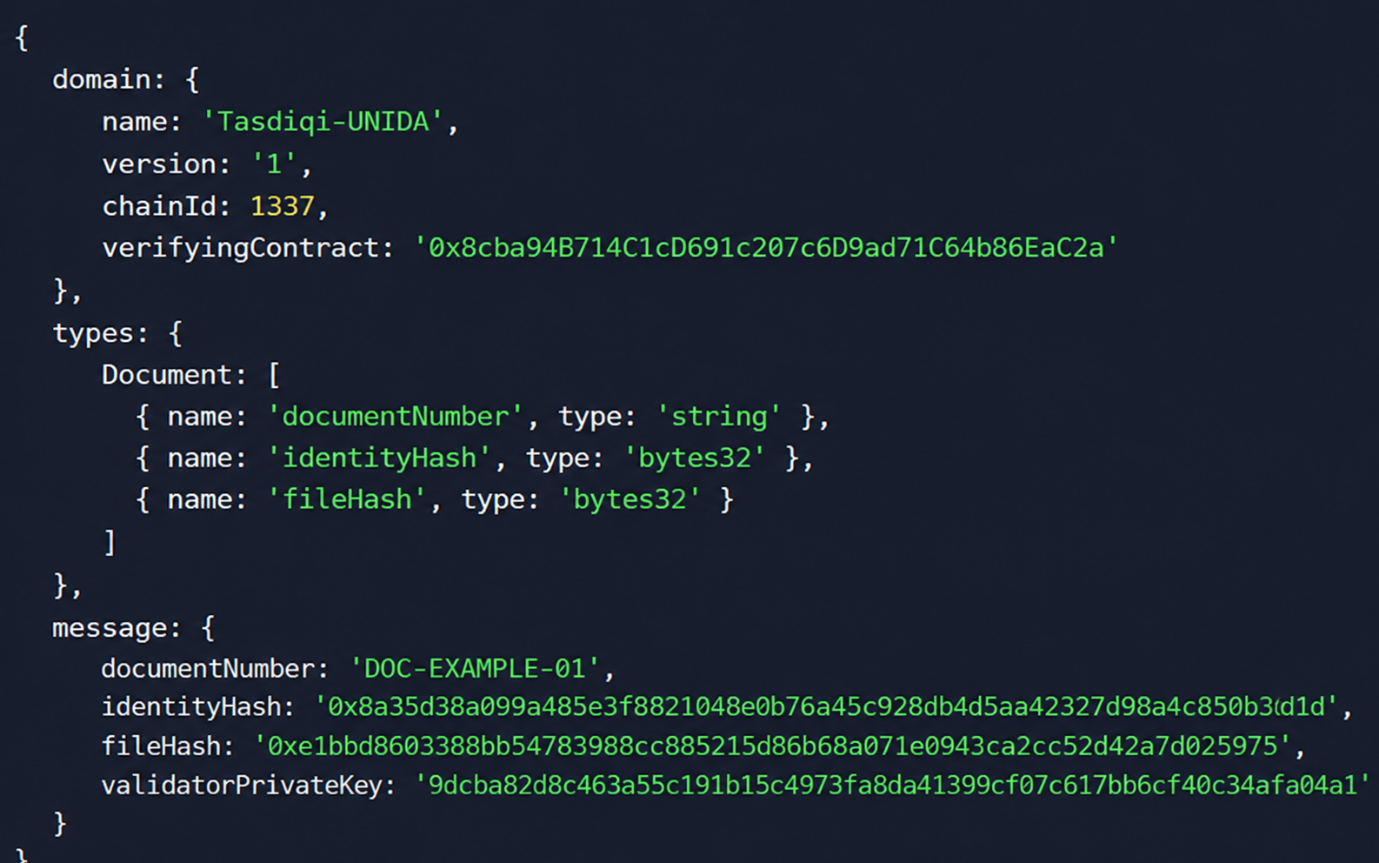
\includegraphics[width=1\textwidth]{assets/eip-712.png}
			\caption{Log EIP-712}
			\label{fig:eip-712}
		\end{figure}

		Berdasarkan hasil tangkapan layar di terminal API Middleware pada gambar \ref{fig:eip-712}, sistem berhasil menampilkan struktur data EIP-712 secara utuh sesaat sebelum proses penandatanganan dilakukan. Dengan rincian analisisi nilai parameter berikut:

		\begin{subsecenumerate}
			\item \textit{Domain}: Bagian ini mengunci konteks penandatanganan agar tidak dapat disalah gunakan pada lingkungan lain. Berdasarkan log, parameter didefinisikan sebagai ‘Tasdiqi-UNIDA’, versi ‘1’, dan chainId 1337, serta alamat kontrak \textit{0x8cba94B714C1eD691c207c6d9ad71C64b86EAc2a}. 
			\item \textit{Types}: Menentukan stuktur tipe data untuk dokumen. Skema ini membatasi bahwa objek dokumen wajib memiliki stuktur data yang sama, pembatasan ini mencegah serangan modifikasi tipe data pada saat rekontruksi data on-chain
			\item \textit{Message}: Berisi data rill dokumen. Berdasarkan log, dokumen yang diproses membawa ‘XXX’, nilai \textit{identityHash} berupa \textit{0x8a35d38a099a485e3f8821048e0b76a45c928db4d5aa42327d90a4c850b3dd1d}, serta nilai \textit{fileHash} berupa \textit{0xe1bbd8603388bb54783988cc885215d86b08a07fe0943ca2cc52d42a7d025975}. Selain itu terekan pula parameter \textit{validatorPrivateKey} yang merupakan kunci privat yang akan bertindak sebagai entitas penandatanganan utama.
		\end{subsecenumerate}

		\subsection{Implementasi Middleware API}

		\begin{figure}[H]
			\centering
			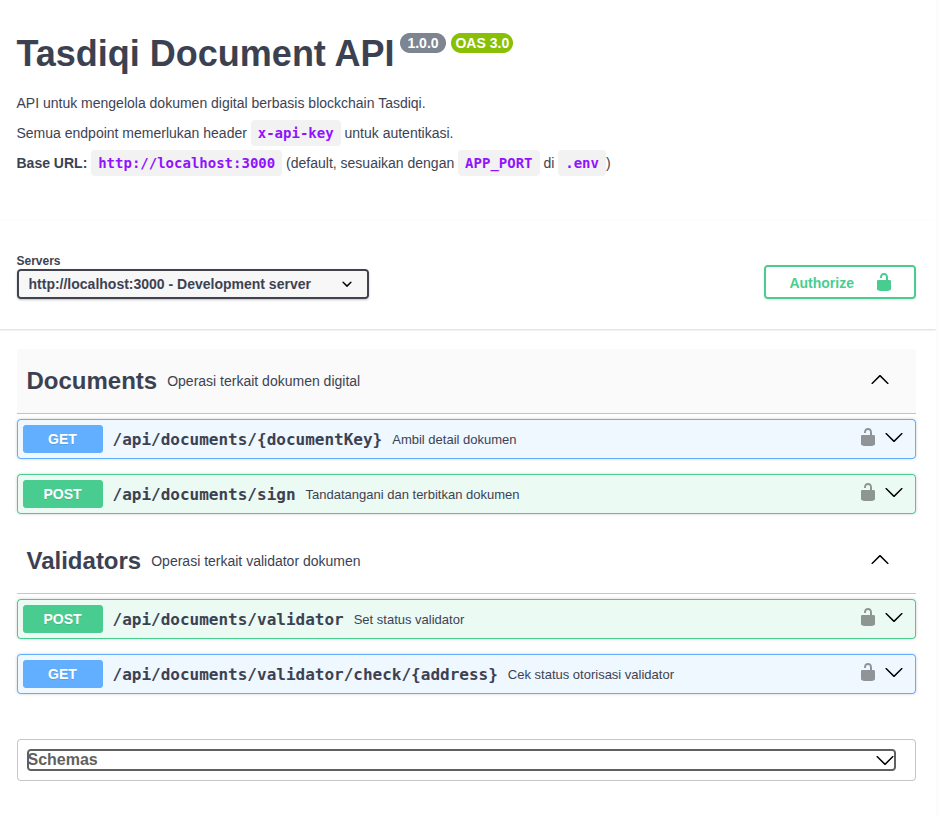
\includegraphics[width=1\textwidth]{assets/swagger-api.png}
			\caption{Dokumentasi API Middleware}
			\label{fig:swagger-api}
		\end{figure}

		Gambar \ref{fig:swagger-api} menampilkan antarmuka dokumentasi \textit{API Middleware} berbasis OpenAPI, dokumen ini terbagi menjadi dua kelompok utama, yaitu kelompok Documents yang menangani pengambilan detail dokumen dan penandatanganan dokumen, dan kelompok validators yang berfungsi untuk menambahkan validator dokumen.

		\subsection{Implementasi Aplikasi Klien}

		\begin{figure}[H]
			\centering
			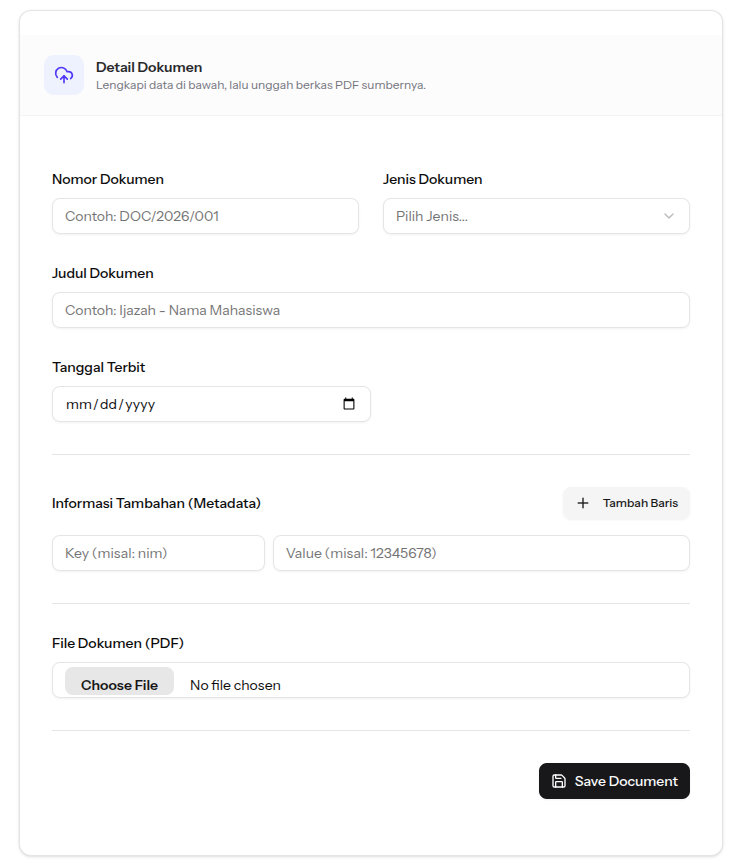
\includegraphics[width=1\textwidth]{assets/upload-dokumen-asli.png}
			\caption{Halaman Upload Dokumen Awal}
			\label{fig:upload-dokumen-asli}
		\end{figure}

		Gambar \ref{fig:upload-dokumen-asli} menunjukan halaman untuk upload dokumen asli sebelum dilakukan penandatanganan, halaman tersebut juga menampilkan informasi pendukung (\textit{metadata}) seperti nomor dokumen, jenis dokumen, judul dokumen, tanggal terbit, serta data tambahan yang dinamis

		\begin{figure}[H]
			\centering
			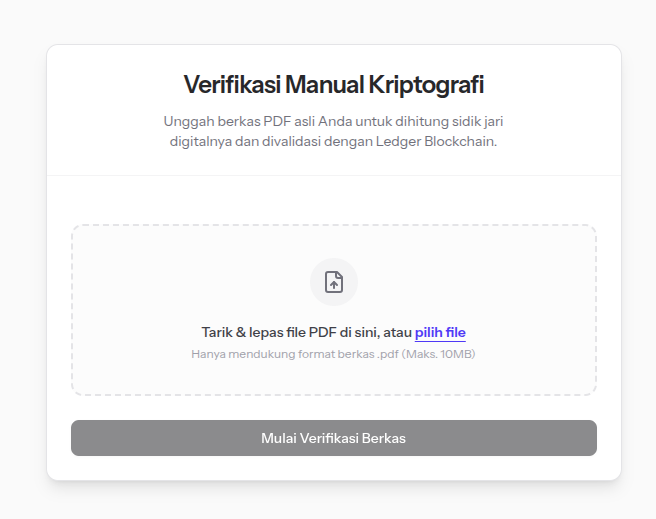
\includegraphics[width=1\textwidth]{assets/upload-manual.png}
			\caption{Halaman Upload Manual}
			\label{fig:upload-manual}
		\end{figure}
		Gambar \ref{fig:upload-manual} menampilkan antarmuka komponen verifikasi manual dengan mengupload dokumen yang akan diverifikasi. Pada implementasinya , antarmuka ini menyediakan area unggah berkas interaktif yang mendukung drag and drop maupun pencarian berkas secara manual, nantinya sistem akan menghitung ulang nilai hash dari dokumen yang di upload kemudian akan dilakukan pencocokan data dari database lokal dengan data di blockchain.
		
		\colorbox{yellow}{GAMBAR DOKUMEN YANG SUDAH ADA QRnya} 
		
		\begin{figure}[H]
			\centering
			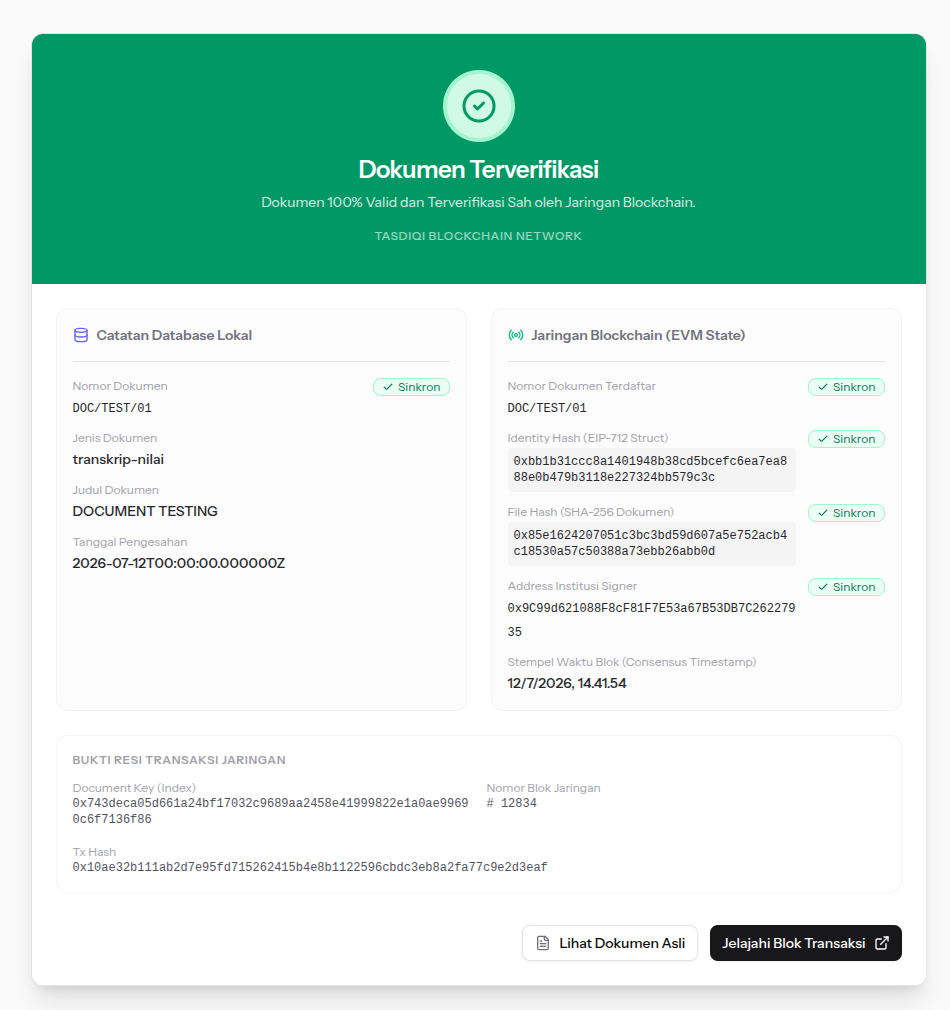
\includegraphics[width=1\textwidth]{assets/verify.png}
			\caption{Halaman Verifikasi}
			\label{fig:verify}
		\end{figure}
		
		Gambar \ref{fig:verify} menampilkan antramuka halaman pengguna verifikasi  sistem yang menunjukan dokumen terverifikasi secara valid dan sah. Pada implementasinya, halaman ini melakukan pencocokan data secara real-time denan membandingkan data di database lokal dengan data pada jaringan blockchain. Status sinkron menandakan bahwa dokumen terbuktu identik dan tidak mengalami manipulasi, yang diperkuat lagi dengan adannya informasi bukti resi transaksi jaringan blockchain
		
	\section{Hasil Pengujian Sistem}

		\subsection{Pengujian Unit Test}
		Pada sub-bab ini, dilakukan pengujian unit (Unit Testing) terhadap API Middleware untuk memastikan semua fungsi autentikasi dan validasi keamanan berjalan sesuai spesifikasi sebelum permintaan diteruskan ke endpoint utama. Pada tabel \ref{tab:pengujian_endpoint_api}  endpoint pengujian diawali dengan prefix \textit{/api/documents}.
	
		% TABLE
		\begin{landscape}

			\renewcommand{\arraystretch}{1.3}

			\begin{longtable}{|
				>{\centering\arraybackslash}p{0.7cm}|
				>{\raggedright\arraybackslash}p{4.3cm}|
				>{\centering\arraybackslash}p{1.8cm}|
				p{6.3cm}|
				p{5.6cm}|
				>{\centering\arraybackslash}p{1.5cm}|}

				\caption{Hasil Pengujian Unit Test API Middleware}
				\label{tab:pengujian_endpoint_api} \\

				\hline
				\textbf{No} &
				\textbf{Endpoint} &
				\textbf{HTTP Method} &
				\textbf{Hasil Uji} &
				\textbf{Ekspektasi} &
				\textbf{Status} \\ \hline
				\endfirsthead

				\hline
				\endfoot

				\hline
				\endlastfoot

				1 &
				\path{/:documentKey} &
				GET &
				Mengambil detail data dokumen digital berdasarkan \textit{document key} yang valid. &
				Mengembalikan objek detail dokumen. &
				Lolos \\ \hline

				2 &
				\path{/sign} &
				POST &
				Melakukan tanda tangan digital dan menerbitkan dokumen ke jaringan \textit{blockchain}. &
				Mengembalikan detail resi transaksi. &
				Lolos \\ \hline

				3 &
				\path{/validator} &
				POST &
				Melakukan registrasi atau pengaktifan status otorisasi alamat validator baru. &
				Mengembalikan \textit{hash} transaksi aktivasi berstatus sukses. &
				Lolos \\ \hline

				4 &
				\path{/validator/check/:address} &
				GET &
				Memeriksa status otorisasi validator pengguna untuk alamat yang sudah terdaftar. &
				Mengembalikan status otorisasi bernilai \textit{isAuthorized: true}. &
				Lolos \\ \hline

			\end{longtable}
		\end{landscape}

		\subsection{Pengujian Blackbock}
		Pengujian \textit{black-box} pada tahap ini dilakukan untuk menguji sistem dari segi fungsionalitas tanpa perlu mengetahui stuktur kode program atau alur logika internal yang ada didalamnya.

			\renewcommand{\arraystretch}{1.3}
			\begin{longtable}{|
				>{\centering\arraybackslash}p{0.8cm}|
				>{\raggedright\arraybackslash}p{2.3cm}|
				p{3.8cm}|
				p{4.5cm}|
				>{\centering\arraybackslash}p{1.6cm}|}

				\caption{Hasil Pengujian Fitur Aplikasi}
				\label{tab:pengujian_fitur} \\

				\hline
				\textbf{No} &
				\textbf{Fitur} &
				\textbf{Kondisi} &
				\textbf{Hasil Uji} &
				\textbf{Status} \\ \hline
				\endfirsthead

				\hline
				\textbf{No} &
				\textbf{Fitur} &
				\textbf{Kondisi} &
				\textbf{Hasil Uji} &
				\textbf{Status} \\ \hline
				\endhead

				\hline
				\endfoot

				\hline
				\endlastfoot

				1 &
				Generate Wallet &
				Admin melakukan generate wallet yang akan digunakan sebagai validator &
				Wallet berhasil dibuat beserta \textit{public address} dan \textit{private address} &
				Berhasil \\ \hline

				2 &
				Upload Dokumen &
				Petugas arsip mengunggah dokumen PDF beserta metadata &
				Dokumen terimpan dan \textit{hash} dokumen berhasil dibentuk &
				Berhasil \\ \hline

				3 &
				Penerbitan Dokumen (EIP-712) &
				Dokumen berhasil diterbitkan dengan validator yang sah &
				Signature berhasil dibuat dan transaksi berhasil dicatat di blockchain &
				Berhasil \\ \hline

				4 &
				Verifikasi QR Code &
				Pengguna memindai QR Code pada dokumen &
				Sistem berhasil mengambil data blockchain dan menampilkan status keaslian dokumen &
				Berhasil \\ \hline

				5 &
				Verifikasi Upload Dokumen &
				Pengguna mengunggah dokumen PDF untuk diverifikasi &
				Sistem menghitung ulang \textit{identityHash} dan \textit{fileHash}, kemudian membandingkannya pada data blockchain &
				Berhasil \\ \hline

			\end{longtable}

		\subsection{Pengujian Validitas Tanda Tangan Digital EIP-712}
		Pengujian kebsahan tanda tangan digital dilakukan untuk memastikan bahwa mekanisme penandatanganan menggunakan standar EIP-712 telah mengehasilkan tanda tangan digital yang valid dan dapat diverifikasi. Berdasarkan spesifikasi EIP-712\footcite{bloemen2017eip712}, data terstuktur harus ditandatangani menggunakan domain separator dan tipe data (\textit{typed structured data}), sehingga identitas dapat dipulihkan kembali dari nilai tanda tangan yang dihasilkan

			% TABLE
			\begin{landscape}

			\renewcommand{\arraystretch}{1.4}

			\begin{table}[!h]
				\centering
				\caption{Hasil Pengujian Keabsahan \textit{Digital Signature} EIP-712}
				\label{tab:pengujian_eip712}

				\begin{tabular}{|
				>{\centering\arraybackslash}p{0.8cm}|
				>{\centering\arraybackslash}p{3.5cm}|
				p{6cm}|
				p{8cm}|
				>{\centering\arraybackslash}p{1.8cm}|}
				\hline

				\textbf{No} &
				\textbf{Komponen yang Diuji} &
				\textbf{Data Uji} &
				\textbf{Nilai Ekspektasi} &
				\textbf{Status} \\ \hline

				1 &
				\textbf{Domain} &
				Parameter \textit{name}, \textit{version}, \textit{chainId}, dan \textit{verifyingContract}. &
				Seluruh parameter \textit{Domain} berhasil dibentuk sesuai konfigurasi jaringan Hyperledger Besu. &
				Lolos \\ \hline

				2 &
				\textbf{Types} &
				Struktur data \texttt{Document} yang terdiri dari \textit{documentNumber} (string), \textit{identityHash} (bytes32), dan \textit{fileHash} (bytes32). &
				Nama setiap field beserta tipe datanya sesuai dengan spesifikasi EIP-712. &
				Lolos \\ \hline

				3 &
				\textbf{Message} &
				\textit{documentKey}, \textit{identityHash}, dan \textit{fileHash}. &
				Data yang akan ditandatangani identik dengan data dokumen yang dikirimkan ke middleware. &
				Lolos \\ \hline

				4 &
				\textbf{Digital Signature} &
				Proses \textit{signTypedData()} terhadap kombinasi \textit{Domain}, \textit{Types}, dan \textit{Message}. &
				\textit{Digital Signature} berhasil dihasilkan sesuai mekanisme EIP-712. &
				Lolos \\ \hline

				5 &
				\textbf{Signer Verification} &
				Alamat hasil \textit{recover} dari \textit{digital signature}. &
				Alamat hasil \textit{recover} identik dengan alamat validator dari arsip sebagai \textit{signer}. &
				Lolos \\ \hline

				\end{tabular}

			\end{table}

			\end{landscape}

		\subsection{Pengujian Validasi Transaksi BLockchain}
		

		\subsection{Pengujian Integritas Dokumen}

		\subsection{Pengujian Zero-Gas Transaction}

	\section{Pembahasan}
	Berdarkan hasil implementasi dan pengujian yang telah dilakukan, dapat disimpulkan bahwa sistem verifikasi dokumen akademik berbasis blockchain berhasil dikembangkan sesuai dengan tujuan penelitian. Integrasi antara aplikasi klien, API Middleware, smart contract, dan jaringan blockchain Hyperledger Besu berjalan dengan baik, sehingga proses penerbitan dan verifikasi dokumen dapat dilakukan secara terstuktur. Hasil penngujian blackbox menunjukan bahwa seluruh fitur utama sistem telah berfungsi sesuai dengan kebutuhan yang telah ditetapkan.

	Lebih lanjut, implementasi protokol EIP-712 berhasil memberikan mekanisme autentikasi terhadap proses penerbitan dokumen melalui tanda tangan digital, sedangkan penggunaan identityHash dan fileHash memungkinkan sistem mendeteksi perubahaan pada file dan metadata berkas melalui perhitungan ulang hash dan pencocokan data yang tersimpan pada blockchain. Selain itu, sistem juga menyediakan dua metode verifikasi, yaitu melalaui QR Code dan unggah dokumen PDF.

	Secara keseluruhan, penelitian ini menunjukan bahwa penerapan blockchain menggunakann Hyperledger Besu dan protokol EIP-712 mempu meningkatkan keamanan, integritas, dan keaslian dokumen akademik. Meskipun demikian, sistem yang dikembangkan masih berupa prototype dan infrastruktur blockchain masih dijalankan pada lingkungan lokal, sehingga penerapan lebih lanjut diperlukan agar dapat diintegrasikan dengan SIAKAD Unida, serta didukung oleh infrastuktur blockchain yang lebih siap diterapkan di lingkungan produksi
		